\chapter{Simulation}

Monte Carlo simulation was used to validate the event selection algorithms
and estimate the energy cut efficiencies and uncertainty.
Two independent simulation programs were developed to achieve these goals.

A simplified Monte Carlo simulation was developed to model the structure
of the Daya Bay data stream \cite{dyb_toymc, dyb_toymc_docdb}.
Rather than simulating the details of physical processes such as scintillation,
neutron capture, and electronics response,
the simplified Monte Carlo used parametrized distributions
to determine the most relevant AD-level observables including the event timestamp
and reconstructed energy and position.
This simulation was configured to match various assumptions
about the Daya Bay data model,
such as a particular rate of uncorrelated events,
or the presence or absence of a certain background.
The resulting output data sets could then be analyzed
to determine the validity of the analysis
under the input configuration.
Data sets could be generated with different assumptions
about time correlations or position distributions,
and impact of those assumptions on the final analysis could be assessed.
However, due to its simplified nature,
the simulation was not able to provide insights about the distributions themselves.

A second, more detailed, Monte Carlo simulation was used
to investigate the detector's response to individual events\todo{cite THU MC}.
This simulation included detailed tracking of individual energy depositions,
scintillator response, and particle interactions such as positron annihilation.
The resulting data sets consisted of detailed information about individual
simulated IBD events,
such as the incident \nuebar{} energy, the target volume (LS or GdLS),
neutron kinetic energy, etc.,
as well as the reconstructed position and energy
based on the simulated electronics response.
This data set could be used to extract efficiencies
by computing the fraction of simulated events which satisfied
various analysis cut criteria.

The detailed simulation produced each event independently,
and did not attempt to simulate the actual Daya Bay data files
containing multiple types of events with various time correlations.
Thus each simulation had a specialized domain,
and both were necessary to complete the analysis.
The simplified simulation was able to answer questions about the more complicated
event selection procedures such as determining the accidental background
or the \li{} and \he{} contamination (\cref{sec:acc,subsec:li9}),
and the detailed simulation was able to estimate
the prompt and delayed energy cut efficiencies (\cref{sec:energy_cuts}).
The details of the simplified and detailed simulations will be described
in \cref{sec:toymc,sec:thu_toymc}, respectively.
A sample of studies that relied on the simulations will be presented
in \cref{sec:toymc_studies,sec:thu_toymc_studies}.

\section{Simplified Monte Carlo}
\label{sec:toymc}

The primary purpose of the simplified Monte Carlo
is for determining the efficiency and effectiveness of the event selection.
In practice, the simulation was used to generate data sets
containing ``idealized'' versions of various event types
(with known energy distribution, no fluctuations, no electronics effects, etc.),
with the same data file format as the actual Daya Bay data files,
so that they can be processed using exactly the same software pipeline
as the real data.
These data sets were then studied to determine how the event selection procedure
performs under ideal circumstances.
The configuration could be varied to, for example,
increase the rate of a particular background process,
or tighten the position correlation between IBD prompt and delayed events,
and the effect of that change could be studied.

The simulation is based on a core set of event types:
Single, Correlated, and Muon.
Additional event types such as Flasher and \li{} were added to support specific studies
(see \cref{sec:toymc_studies}).
The simulation's configuration allows for customization of the event rate
for each different event type,
and also for multiple variants of the event type.
For example, one type of Correlated event could be configured to represent nH IBDs,
and a second type could be configured to represent nGd IBDs
with a shorter coincidence time, higher delayed energy,
and with the delayed event position limited to the GdLS (IAV) region of the AD.

When the simulation is executed,
the appropriate number of each type of event is generated
based on the desired time interval to be simulated.
The events are then saved to disk in the same ROOT file data format
used by the Daya Bay data production.
An additional ROOT TTree structure containing the ``truth information''
for each event is included in the output data file.
For this simulation, the only ``truth'' hidden from the data output
is the event type that the given data entry represents.
The characteristics associtated with the different event types
are described below.

\subsection{Types of generated events}

Single events represent uncorrelated signals,
which in Daya Bay are mostly due to natural radioactive decays in the AD
(\cref{subsec:singles}).
In the simulation, Single events are assigned timestamps
drawn uniformly at random between the time limits given in the configuration,
representing their uncorrelated nature.
The event energies are also drawn uniformly at random
between \SIlist{1;3.5}{\MeV},
and the positions are similarly randomly assigned
within the OAV cylinder.

Correlated events represent pairs of signals
with a common physical origin, both in position and in time.
IBDs and correlated backgrounds (\cref{sec:correlated_bg})
satisfy these criteria for being modeled by the Correlated event type.
To create the time correlation between prompt and delayed events,
modeled as an exponential distribution,
the simulation first determines the timestamp for a prompt event at random.
Then the coincidence time delay between prompt and delayed events is generated
from an exponential distribution
whose time constant is specified in the simulation configuration.
The prompt and delayed energies are determined independently at random
using uniform distributions specified by the simulation configuration.
The position of the prompt event is chosen at random
within the GdLS or LS volumes (again, as specified by the configuration),
and the delayed position is chosen to be correlated with the prompt position.
Since exact modeling of the position correlations is not crucial,
a simple exponential distribution is used to determine the displacement
in each direction ($x,y,$ and $z$) for these Correlated events.
In the recorded truth information,
prompt and delayed events are assigned separate labels
even though they both form part of the same Correlated event type.

Muon events represent signals created by muons traversing
the water pools and ADs (\cref{sec:muonveto}).
For simplicity, each muon is assumed to create a signal
in the inner water pool with probability \num{1}.
The rates and energies were chosen to approximately model
the true distributions and rates of muon signals in the near halls (EH1 and EH2).
A portion of the muon signals, \SI{19.95}{\percent},
traverse the AD, depositing an energy chosen at random between
\SIlist{20;2000}{\MeV}.
A smaller subset of the muon signals, \SI{0.05}{\percent},
create particle showers in the AD, depositing an energy chosen at random between
\SIlist{2500;5000}{\MeV}.
The time delay between WP and AD muons is assigned to be \SI{50}{\ns},
chosen since in real data there a nonzero time offset between WP and AD muons,
but the distribution of time offsets
is not a critical feature of the event selection.
All of the choices of energies and rates are approximations
designed to capture the general behavior of muons at Daya Bay
without adding excessive complexity to the simulation.

\section{Studies with the simplified Monte Carlo}
\label{sec:toymc_studies}
\subsection{Study of uncorrelated event rate}

The procedure for determining the uncorrelated event rate
is described in \cref{subsec:singles}.
This process, both the abstract procedure and the actual software implementation,
was validated using simulated datasets.
The simulation was configured to generate Single (uncorrelated) events
with a rate of \SI{20}{\Hz}
in data files also containing Muon and Correlated events.
The full configuration is listed in \cref{tab:toymc_singles_config}.
The simulation was used to generate 100 data sets,
each consisting of 300 files containing 10 minutes' worth of data,
for a total of 50 hours of data per data set.
The data files were processed using the event selection software
and an empirical rate for uncorrelated events was extracted
for each of the 100 data sets.
The distribution of measured uncorrelated event rates
is shown in \cref{fig:toymc_singles_dist}.
The mean singles rate was \SI{19.9935+-0.0013}{\Hz}
which is a bias of \SI{0.033}{\percent} (5 standard deviations)
relative to the ``true'' input rate.
\todo[inline]{Explain why such a small bias is an issue}

%The bias in the measured uncorrelated event rate,
%if also present in the real Daya Bay data,
%would have led to an underestimation of accidental coincidence events in each AD.
%The final extracted IBD rate therefore would have been slightly higher
%than the actual IBD rate in each AD,
%by approximately the same number of IBDs per day per AD,
%(since the singles rate and therefore accidental rate
%is approximately the same in each AD).
%This affine scaling would have lessened the apparent deficit of IBDs
%between the near and far halls,
%thus biasing the measurement of \thetaot.

It was hypothesized that the bias was due to an unintended effect
of the absolute fixed input event rate,
which does not fluctuate according to Poisson statistics in the simulation.
Each simulated 10-minute data file has precisely the same number of uncorrelated events,
which violates the assumption that the number of events follows the Poisson distribution.
Specifically, at an uncorrelated event rate of \SI{20}{\Hz},
each file contains exactly \num{12000} uncorrelated events.
If the occurrence of uncorrelated events were truly random,
then each 10-minute file should expect fluctuations of approximately
$\sqrt{12000} = 110$~events or \SI{0.09}{\percent}.
The impact of the absence of these fluctuations
on the probability of an accidental coincidence is complex;
therefore, an additional simulation was performed
to assess the impact.
If individual data files were longer, then the relative size of fluctuations,
and therefore any impact on the measured singles rate,
should be suppressed.
A second set of 100 data sets was generated to test this hypothesis,
where each data set was a single 1000-minute data file.
The distributrion of measured uncorrelated event rates from this second data set
is shown in \cref{fig:toymc_singles_dist}.
There was a larger spread due to the shorter duration of each data file,
but the mean over all 100 data sets was \SI{19.9966+-0.0022}{\Hz},
which is a bias of \SI{0.017}{\percent} or 2 standard deviations.
The bias decreased as the length of the simulated data file increased
(even as the number of events in the data set decreased),
suggesting that the origin of the bias is related to the length of the simulated files.
Thus the simulation was able to confirm that
the event selection software can successfully extract
the uncorrelated event rate with high precision and minimal bias.

\begin{table}[ht]
    \centering
    \begin{tabular}[t]{llll}
        \hline
        Event type & {Rate [\si{\Hz}]} & Energy [\si{\MeV}] & Coincidence time [\si{\us}]\\
        \hline
        Single & \num{20} & $[\num{1.5}, \num{3}]$ & -\\
        \multirow{2}{*}{Correlated (nH)}
               & \multirow{2}{*}{\num{0.005}}
               & [\num{0.7}, \num{4}] (prompt)
               & \multirow{2}{*}{\num{150}} \\
               & & [\num{1.9}, \num{2.3}] (delayed) & \\
        \multirow{2}{*}{Correlated (nGd)}
               & \multirow{2}{*}{\num{0.0067}}
               & [\num{0.7}, \num{4}] (prompt)
               & \multirow{2}{*}{\num{28}} \\
               & & [\num{7}, \num{9}] (delayed) & \\
        Water Pool Muon & \num{200} & - & - \\
        AD Muon & \num{39.9} & [\num{20}, \num{2000}] & -\\
        Showering Muon & \num{0.1} & [\num{2500}, \num{5000}] & -\\
    \end{tabular}
    \caption{Simulation configuration inputs for the uncorrelated event rate study.}
    \label{tab:toymc_singles_config}
\end{table}

\begin{figure}
    \centering
    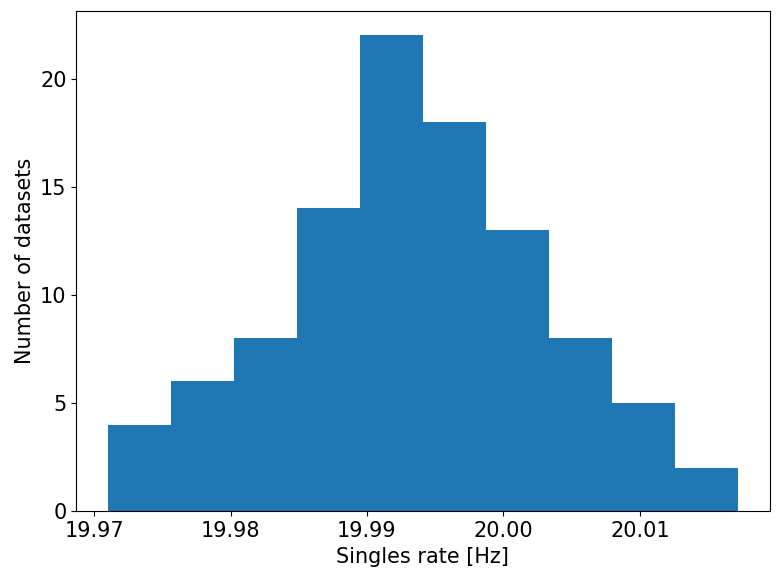
\includegraphics[width=0.7\textwidth]{ch_simulation/singles_rate_dist}
    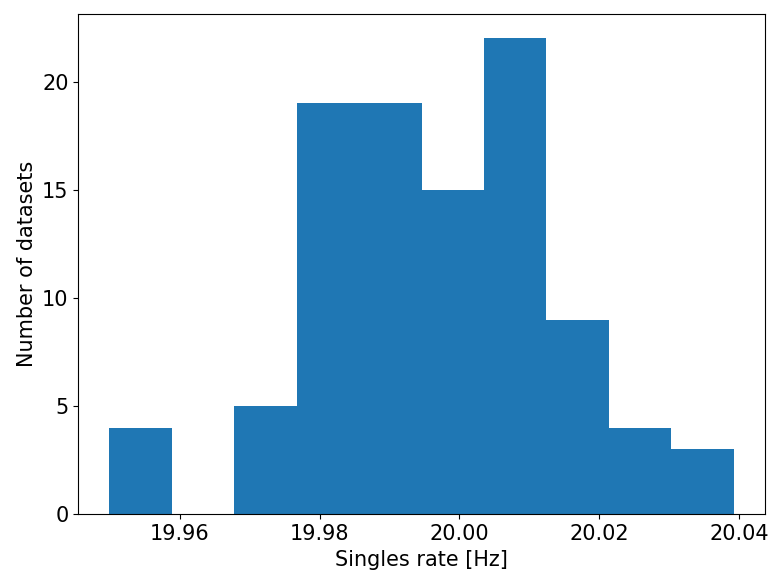
\includegraphics[width=0.7\textwidth]{ch_simulation/singles_rate_unbiased_dist}
    \caption{
        Distribution of uncorrelated event rates over 100 simulated data sets.
        The simulation configuration (``truth'') specified a rate of \SI{20}{\Hz}.
        Top: Each data set consists of 300 data files, each with 10 minutes of data.
        Bottom: Each data set consists of a single 1000-minute data file.
    }
    \label{fig:toymc_singles_dist}
\end{figure}

\subsection{Muon-induced isotopes}
\label{subsec:toymc_li9}

The Muon event type was augmented to provide validation
of the software used to search for decays of muon-induced isotopes
(\cref{subsec:li9}).
In addition to generating water pool, AD and showering muons,
the simulation also generated muon-correlated neutrons
and muon-correlated unstable isotope decays
meant to represent \li{} and \he.
The analysis software identified a muon as neutron-tagged
if it was followed by a neutron-like signal
with a delay of between \SIlist{20;200}{\us}.
Since the truth labels recorded whether a muon signal
was accompanied by a neutron tag,
the list of neutron-tagged muons found by the analysis software
could be compared with the list of ``true'' neutron-tagged muons
to validate the functionality of the neutron tagger.
\todo[inline]{Update when Li-9 analysis is more mature}

\subsection{Flashers}
\label{subsec:toymc_flashers}

Light emission by PMTs caused a background of single events
known as flashers (\cref{sec:flashers}).
The vast majority of flasher events are rejected using an event-by-event veto,
and the remaining flashers are assumed to be accounted for
by the treatment of the accidental background (\cref{sec:acc}).
Certain PMTs were observed to flash with a frequency
of approximately \SI{0.1}{\Hz},
but with the restriction that
the same PMT will never flash twice within $\sim$\SI{0.3}{\s}.
This pattern breaks the assumption in the accidental background analysis
that all single events are uncorrelated and governed by Poisson statistics.
A Flasher event type was added to the simulation to test the impact of this deviation.

The Flasher event type had a fixed energy
and generated events were given fixed, deterministic timestamps \SI{1}{\s} apart.
A data sample was generated with only Single events and Flasher events,
and was treated as if the Flasher events passed the existing flasher veto criteria.
The accidental background analysis was performed on this data sample,
with the expected output of \num{0} coincident events remaining
after subtracting the accidental background.
However, the actual output number of events was negative.
Further inspection showed that the residual flasher events,
like all other single events,
contributed to the synthetic accidentals sample,
and in that sample some of the pairs
were composed of two residual flasher events.
In the real (simulated) data set, though,
there were no accidental coincidences between residual flashers by construction,
since the residual flasher events were generated with \SI{1}{\s} time gaps
between consecutive flashers.
\todo[inline]{Add more when Olivia reports back}

\section{Detailed Monte Carlo}
\label{sec:thu_toymc}

\section{Studies using the detailed Monte Carlo}
\label{sec:thu_toymc_studies}

\subsection{Prompt energy efficiency}
\label{subsec:thu_toymc_prompt}

The detailed Monte Carlo was used to estimate the prompt energy efficiency,
the fraction of IBD events whose reconstructed prompt energy
satisfied the prompt energy criterion of $E > \SI{1.5}{\MeV}$
(\cref{subsec:prompt_energy}).
The spectrum of reconstructed energy for the Monte Carlo sample of IBD prompt events
is shown in \cref{fig:prompt_eff_mc}.
The prompt energy cut efficiency is the fraction of events in the histogram
with energy above \SI{1.5}{\mev}.
\todo[inline]{Fill in details of absolute efficiency determination}

The AD-uncorrelated uncertainty on the prompt energy efficiency
was also determined using the simulation.
Each AD has a slightly different relative energy scale (\cref{subsec:rel_energyscale}),
resulting in different fractions of IBD prompt events
being assigned a reconstructed energy above \SI{1.5}{\MeV}.
The relative energy scale variation was measured to be \SI{+-0.5}{\percent},
and this effect was reproduced by simply
scaling the reconstructed energy for each simulated event by \SI{+-0.5}{\percent}.
The variation in efficiency due to this re-scaling,
and therefore the AD-uncorrelated relative uncertainty on the prompt energy efficiency,
was \SI{+-0.1}{\percent}.

\begin{figure}
    \centering
    \includegraphics[width=0.49\textwidth]{%
        ch_event_selection/prompt_energy_mc%
    }
    \includegraphics[width=0.49\textwidth]{%
        ch_event_selection/delayed_energy_mc%
    }
    \caption{The spectrum of reconstructed energy for simulated IBD prompt (left)
        and delayed (right) events
        in the Monte Carlo study used to compute the prompt and delayed
        energy cut absolute efficiencies.
        The prompt spectrum is also used to compute the prompt energy cut
    efficiency AD-uncorrelated uncertainty.}
    \label{fig:prompt_eff_mc}
\end{figure}
